\section{System Architecture}

\begin{figure}[h]
  \centering
  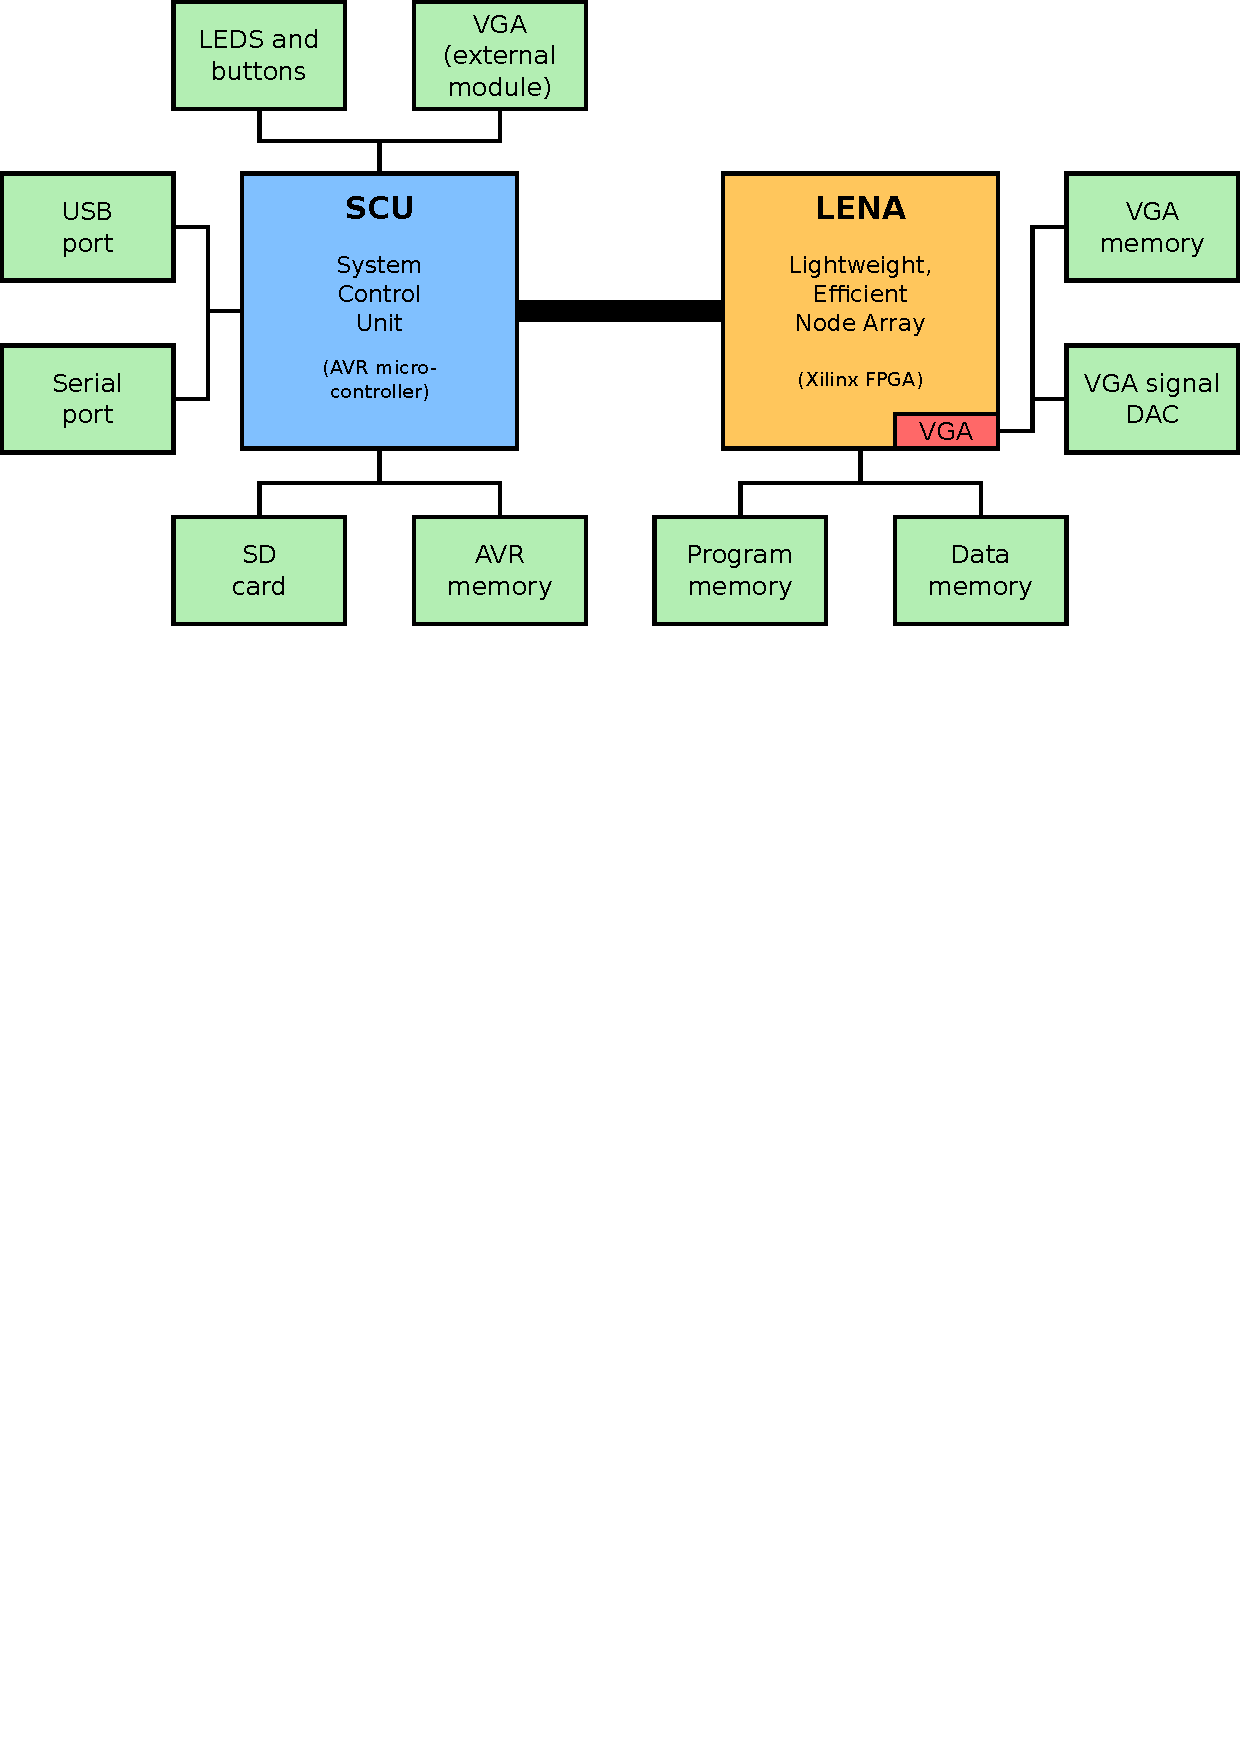
\includegraphics[width=\linewidth,clip,trim=0 18cm 0 0]
                  {fig/sys-over/arch-fig.pdf}
  \caption{System Architecture}
  \label{fig:sys-over-arch-fig}
\end{figure}


A general concern when designing large systems is the accidental
complexity\cite[p.~8-9]{holt2004uml} one may create by poor design choices early
on. Many solutions designed to reduce accidental complexity are based around
software systems, and sacrifices performance in both the time domain and in the
space domain\cite{moseley2006out}. While these solutions may be applicable
within hardware systems where these kinds of performance degradations are not a
problem, it is unacceptable in systems where one or multiple of the system
requirements are a performance increase in one or both of these domains. As one
of our main requirements is focus on performance, we have to accept a certain
level of inherent complexity.

To remedy the complexity which comes from our requirements, we focused on making
it possible to isolate errors and make it possible to test the individual
components as fast as possible: The LENA architecture was tested through VHDL
test benches, the VGA component in the LENA architecture was tested directly on
the board, and the AVR part of the system tested different input and output
devices directly on the board.\TODO{Is this, hmm \ldots stating the obvious?} By
doing this, we can ensure that errors occuring when connecting different
components is due to errors in the protocol implementation.

Figure \ref{fig:sys-over-arch-fig} shows our resulting architecture. Buttons and
LEDs made it easy to confirm that the VGA operates properly for simple
programs. A VGA connector made it possible to quickly test and debug the VGA
implementation on the LENA architecture. We also included a VGA connector
connected to the AVR, in case something would happen with the LENA
implementation.

% TODO: I/O device discussion, memory discussion, word size
To be able to process data, we need an I/O device which serves
